\subsection{Part 2}
\begin{frame}
    \frametitle{Outline}
    \tableofcontents[currentsection]
\end{frame}

\begin{frame}
    \frametitle{Stability theorem proof, part 2}

    We want to prove the limits
    \begin{gather*}
        \lim_{k \rightarrow \infty} \| \hat{\theta}_c(k) - \hat{\theta}_c(k-1) \| = 0 \\
        \, \\
        \lim_{k \rightarrow \infty} \frac{ [\lambda_1(k-1) e^o(k)]^2 }
            { \lambda_1(k-1) + \phi^T(k-\drm) F(k-1) \phi(k-\drm) } = 0 \\
        \, \\
        \lim_{k \rightarrow \infty} \frac{ [\lambda_1(k-1) \epsilon(k)]^2 }
            { \lambda_1(k-1) + \phi^T(k-\drm) F(k-1) \phi(k-\drm) } = 0
    \end{gather*}
\end{frame}

\begin{frame}
    \frametitle{Stability theorem proof, part 2}

    \begin{columns}[c]
        \column{0.55\textwidth}
        We know that $1 - \lambda / 2$ is SPR, which implies that it is P-class

        $ \ $

        This implies that there exists $\bar{\gamma} \in \mathcal{R}$ such that
        \begin{align*}
            -\bar{\gamma}^2 & \leq \sum_{j=0}^k m(j) v(j) \\
            & = - \sum_{j=0}^k w(j) \Big[ s(j) \\
            & \quad + \frac{1}{2}(\lambda - \lambda_2(j-1)) w(j)\Big]
        \end{align*}


        \column{0.45\textwidth}
        \begin{figure}[h]
            \centering
            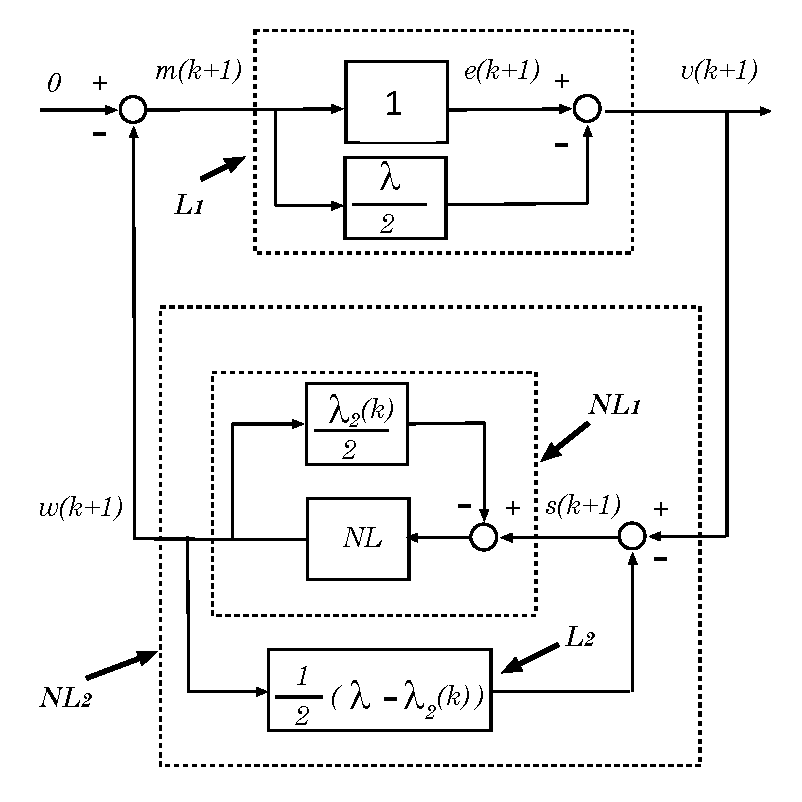
\includegraphics[width=\columnwidth]{figs_hyperstability}\\
        \end{figure}
    \end{columns}
\end{frame}

\begin{frame}
    \frametitle{Stability theorem proof, part 2}

    Because $\lambda - \lambda_2(j-1) \geq 0, \ j = -1,0,1,\ldots$, we have
    \begin{align*}
        -\bar{\gamma}^2 & \leq -\sum_{j=0}^k w(j) \Big[ s(j) + \frac{1}{2}(\lambda - \lambda_2(j-1)) w(j) \Big] \\
        & \leq -\sum_{j=0}^k w(j) s(j) \\
    \end{align*}
    \pause
    which implies that
    \begin{align*}
        \sum_{j=0}^k w(j) s(j) \leq \bar{\gamma}^2
    \end{align*}
\end{frame}

\begin{frame}
    \frametitle{Stability theorem proof, part 2}

    From part 1 of the stability theorem proof,
    \begin{align*}
        2 w(k) s(k) & = \tilde{\theta}_c^T(k) F^{-1}(k) \tilde{\theta}_c(k)
            - \lambda_1(k) \tilde{\theta}_c^T(k-1) F^{-1}(k-1) \tilde{\theta}_c(k-1) \\
        & \quad + \lambda_1(k) \Delta\theta_c^T(k) F^{-1}(k-1) \Delta\theta_c(k)
    \end{align*}
    \pause

    Since $0 < \underline{\lambda}_1 \leq \lambda_1(k) \leq 1$ and $F(k-1) \succ 0$, this implies that
    \begin{align*}
         2 w(k) s(k) & \geq \left[ \tilde{\theta}_c^T(k) F^{-1}(k) \tilde{\theta}_c(k)
            - \tilde{\theta}_c^T(k-1) F^{-1}(k-1) \tilde{\theta}_c(k-1) \right] \\
         & \quad + \underline{\lambda}_1 \Delta\theta_c^T(k) F^{-1}(k-1) \Delta\theta_c(k)
    \end{align*}
        
\end{frame}

\begin{frame}
    \frametitle{Stability theorem proof, part 2}    
    
    \begin{align*}
         2 w(k) s(k) & \geq \left[ \tilde{\theta}_c^T(k) F^{-1}(k) \tilde{\theta}_c(k)
            - \tilde{\theta}_c^T(k-1) F^{-1}(k-1) \tilde{\theta}_c(k-1) \right] \\
         & \quad + \underline{\lambda}_1 \Delta\theta_c^T(k) F^{-1}(k-1) \Delta\theta_c(k)
    \end{align*}
    \hrule{\hfill}
    
    which implies that
    \begin{align*}
        2 \bar{\gamma}^2 & \geq 2 \sum_{j=0}^k w(j) s(j) \\
        & \geq \sum_{j=0}^k \left[ \tilde{\theta}_c^T(j) F^{-1}(j) \tilde{\theta}_c(j)
            - \tilde{\theta}_c^T(j-1) F^{-1}(j-1) \tilde{\theta}_c(j-1) \right] \\
        & \quad + \sum_{j=0}^k \underline{\lambda}_1 \Delta \theta_c^T(j) F^{-1}(j-1) \Delta \theta_c(j)
    \end{align*}
\end{frame}

\begin{frame}
    \frametitle{Stability theorem proof, part 2}

    \vspace*{-\baselineskip}
    \begin{align*}
        2 \bar{\gamma}^2 & \geq \sum_{j=0}^k \left[ \tilde{\theta}_c^T(j) F^{-1}(j) \tilde{\theta}_c(j)
            - \tilde{\theta}_c^T(j-1) F^{-1}(j-1) \tilde{\theta}_c(j-1) \right] \\
        & \quad + \sum_{j=0}^k \underline{\lambda}_1 \Delta \theta_c^T(j) F^{-1}(j-1) \Delta \theta_c(j)
    \end{align*}
    \hrule{\hfill}
    
    \vspace*{-\baselineskip}
    \begin{align*}
        2 \bar{\gamma}^2 & = \tilde{\theta}_c^T(k) F^{-1}(k) \tilde{\theta}_c(k)
            - \tilde{\theta}_c^T(-1) F^{-1}(-1) \tilde{\theta}_c(-1) \\
        & \quad + \underline{\lambda}_1 \sum_{j=0}^k \Delta \theta_c^T(j) F^{-1}(j-1) \Delta \theta_c(j) \\
        & \geq - \tilde{\theta}_c^T(-1) F^{-1}(-1) \tilde{\theta}_c(-1)
            + \underline{\lambda}_1 \sum_{j=0}^k \Delta \theta_c^T(j) F^{-1}(j-1) \Delta \theta_c(j)
    \end{align*}
\end{frame}

\begin{frame}
    \frametitle{Stability theorem proof, part 2}

    Thus, we know that
    \begin{align*}
        \sum_{j=0}^k \Delta \theta_c^T(j) F^{-1}(j-1) \Delta \theta_c(j) \leq
            \frac{1}{ \underline{\lambda}_1 } 
            \left[ 2 \bar{\gamma}^2 + \tilde{\theta}_c^T(-1) F^{-1}(-1) \tilde{\theta}_c(-1) \right]
    \end{align*}
    \pause
    Since $F^{-1}(k) \succ 0 \ \forall k$, this implies that
    \begin{align*}
        \lim_{k \rightarrow \infty} \Delta \theta_c^T(k) F^{-1}(k-1) \Delta \theta_c(k) = 0
    \end{align*}
    \pause

    Since $\displaystyle \lambda_{min} (F^{-1}(k-1)) = \frac{1}{ \lambda_{max} (F(k-1)) } \geq \frac{1}{K_{max}} > 0$, this implies that
    \alignbox{
        \lim_{k \rightarrow \infty} \| \Delta \theta_c(k) \| = 0
    }
\end{frame}

\begin{frame}
    \frametitle{Stability theorem proof, part 2}

    Substituting the parameter update equation
    \begin{align*}
        \Delta \theta_c(k) = F(k-1) \phi(k-\drm) e(k)
    \end{align*}
    into
    \begin{align*}
        \lim_{k \rightarrow \infty} \Delta \theta_c^T(k) F^{-1}(k-1) \Delta \theta_c(k) = 0
    \end{align*}
    we obtain
    \begin{align*}
        \lim_{k \rightarrow \infty} \phi^T(k-\drm) F(k-1) \phi(k-\drm) e^2(k) = 0
    \end{align*}
    \pause
    Adding the equation $\displaystyle \lim_{k\rightarrow \infty} \lambda_1(k-1) e^2(k) = 0$ to this equation yields
    \begin{align*}
        \lim_{k \rightarrow \infty} [\lambda_1(k-1) + \phi^T(k-\drm) F(k-1) \phi(k-\drm)] e^2(k) = 0
    \end{align*}

\end{frame}

\begin{frame}
    \frametitle{Stability theorem proof, part 2}

    We know that
    \begin{align*}
        \lim_{k \rightarrow \infty} [\lambda_1(k-1) + \phi^T(k-\drm) F(k-1) \phi(k-\drm)] e^2(k) = 0
    \end{align*}

    $ \ $

    Since $\displaystyle e(k) = \frac{ \lambda_1(k-1) e^o(k) }{ \lambda_1(k-1) + \phi^T(k-\drm) F(k-1) \phi(k-\drm) } $, we have

    $ \ $

    \alignbox{
        \lim_{k \rightarrow \infty} \frac{ [\lambda_1(k-1) e^o(k)]^2 }
            { \lambda_1(k-1) + \phi^T(k-\drm) F(k-1) \phi(k-\drm) } = 0
    }

\end{frame}

\begin{frame}
    \frametitle{Stability theorem proof, part 2}

    Recall that $\eta_d(k) = r(k-\drm)$ and the control is given by
    \begin{align*}
        \hat{R}(q^{-1},k) u(k) = r(k) - \hat{S}(q^{-1},k) y(k)
    \end{align*}
    \pause
    We therefore see that
    \begin{align*}
        \eta_d(k+\drm) & = r(k) = \hat{R}(q^{-1},k) u(k) + \hat{S}(q^{-1},k) y(k) \\
        & = \phi^T(k) \hat{\theta}_c(k)
    \end{align*}
    \pause
    which allows us to say that
    \begin{align*}
        \epsilon(k) & = \eta(k) - \eta_d(k) = \phi^T(k-\drm) \tilde{\theta}_c(k-\drm) \\
        & = {\color{red} \phi^T(k-\drm) \tilde{\theta}_c(k-1) } + \phi^T(k-\drm) \Big[ \tilde{\theta}_c(k-\drm)
            - \tilde{\theta}_c(k-1) \Big] \\
        & = {\color{red} e^o(k)} + \phi^T(k-\drm) \Big[ \tilde{\theta}_c(k-\drm)
            - \tilde{\theta}_c(k-1) \Big]
    \end{align*}

\end{frame}

\begin{frame}
    \frametitle{Stability theorem proof, part 2}

    For convenience, define

    \begin{align*}
        \zeta(k) = \frac{\lambda_1(k-1) + \phi^T(k-\drm) F(k-1) \phi(k-\drm)}{\lambda_1^2(k-1)}
    \end{align*}
    In this notation, we know that $\displaystyle \lim_{k\rightarrow \infty} \frac{ [e^o(k)]^2 }{ \zeta(k) } = 0$
    \pause
    
    $\,$

    Since $0 < \lambda_1(k) \leq 1$ and $0 < K_{min} \leq \lambda_{min} (F(k)) \ \forall k$, we have
    \begin{gather*}
        \zeta(k) > \phi^T(k-\drm) F(k-1) \phi(k-\drm)
            \geq K_{min} \| \phi(k-\drm) \|^2 \geq 0
    \end{gather*}
    \paused
    
    \begin{gather*}
        \Rightarrow \frac{ \| \phi(k-\drm) \|^2 }{\zeta(k)} < \frac{1}{K_{min}}
    \end{gather*}

\end{frame}

\begin{frame}
    \frametitle{Stability theorem proof, part 2}

    By the Cauchy-Schwarz inequality,
    \begin{align*}
        & \left| \frac{ \phi^T(k-\drm) \Big[ \tilde{\theta}_c(k-\drm) - \tilde{\theta}_c(k-1) \Big] }
            { \sqrt{\zeta(k)} } \right| \\
        & \hspace{2.5cm} \leq \frac{ \| \phi(k-\drm) \| }{ \sqrt{\zeta(k)} } \|
            \tilde{\theta}_c(k-\drm) - \tilde{\theta}_c(k-1) \| \\
        & \hspace{2.5cm} \leq \frac{1}{ \sqrt{K_{min}} }
            \| \tilde{\theta}_c(k-\drm) - \tilde{\theta}_c(k-1) \|
    \end{align*}
    \pause
    
    The right-hand side of this inequality converges to zero because $\| \tilde{\theta}_c(k-\drm) - \tilde{\theta}_c(k-1) \|$ converges to zero.
    \pause
    
    Therefore
    \begin{align*}
        \lim_{k\rightarrow \infty} \frac{ \phi^T(k-\drm) \Big[ \tilde{\theta}_c(k-\drm) - \tilde{\theta}_c(k-1) \Big] }
            { \sqrt{\zeta(k)} } = 0
    \end{align*}

\end{frame}

\begin{frame}
    \frametitle{Stability theorem proof, part 2}

    Since $\epsilon(k) =  e^o(k) + \phi^T(k-\drm) \Big[ \tilde{\theta}_c(k-\drm) - \tilde{\theta}_c(k-1) \Big]$, we have
    \begin{align*}
        \lim_{k \rightarrow \infty} \frac{ \epsilon(k) }{ \sqrt{\zeta(k)} }
            & = \lim_{k \rightarrow \infty} \frac{ e^o(k) }{ \sqrt{\zeta(k)} } \\
        & \quad + \lim_{k \rightarrow \infty} \frac{ \phi^T(k-\drm) \Big[ \tilde{\theta}_c(k-\drm)
            - \tilde{\theta}_c(k-1) \Big] }{ \sqrt{\zeta(k)} } \\
        & = 0 + 0
    \end{align*}
    \pause

    Therefore
    \alignbox{
        \lim_{k \rightarrow \infty} \frac{ [\lambda_1(k-1) \epsilon(k)]^2 }
            { \lambda_1(k-1) + \phi^T(k-\drm) F(k-1) \phi(k-\drm) } = 0
    }

\end{frame}



